\section{Introduction}\label{intro}\sloppy
The availability of data and vast cloud-based computational resources are allowing both industry and academia to build ever more sophisticated machine learning (ML) applications.
The database community has built systems that support almost every stage of the development process including featurization~\cite{keystone,zhang2014mat}, distributed model training~\cite{hellerstein2012madlib, crotty2014tupleware, feng2012towards, tensor}, and model deployment~\cite{crankshawmissing}.  
However, an often under-discussed, yet crucial, part of ML development is managing dirty data.
In the context of ML, dirty data refers to unintended or unpredictable numerical features that arise from a violation of an invariant expected by the developer (e.g., un-handled NULL values being automatically mapped to 0).
Dirty data affects both the model training and any future predictions the application might make, and numerous papers~\cite{sculley2014machine} and surveys of analysts~\cite{kandel2012, krishnan2016hilda} suggest that the effects and costs of dirty data are pervasive.

%that it takes significant effort to manually identify dirty data and design software to mitigate their effects 

\iffalse
\begin{figure}[t]
% \vspace{-5pt}
\centering
 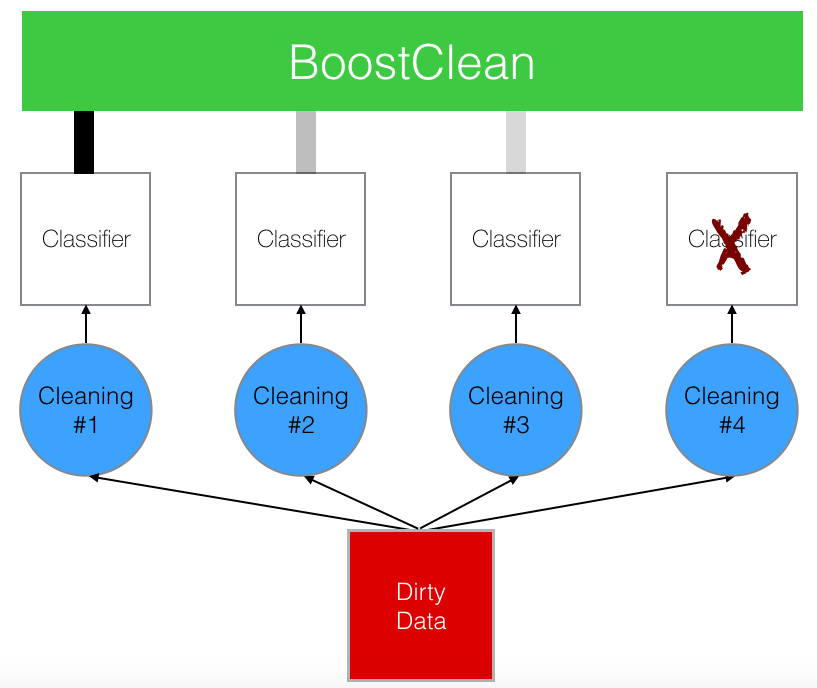
\includegraphics[width=0.8\columnwidth]{figures/teaser.png}
 \caption{ \sys is a new data cleaning system that detects errors in ML data and adaptively selects from a set of repair actions to maximize prediction accuracy. This selection problem is formulated as a statistical boosting procedure, which reweights the data to focus on model mispredictions.
 \label{fig:teaser}}
\end{figure}
\fi

As a concrete example, we are collaborating with a data science company called \company\footnote{Anonymized at the request of the company.} that ranks sales leads. The company aggregates clients' Salesforce.com data on past sales leads, integrates this data with additional information scraped from the web about the client and those leads, and trains a classification model that predicts the success of future uncontacted leads.  Because the data are acquired from a combination of manual data entry and automatically scraped web data, inconsistencies, missing data, and incorrect values are a significant problem.  For instance, a typical error is the inconsistent representation of missing values (e.g., ``-999'', ``EMPTY'' or ``none'' may be used depending on the sales representative).  If the featurization code does not recognize and address these errors, it can lead to biases that degrade the quality of the model. For example, the data scientist may impute a default mean value for all blank attributes but miss the code ``-999'', which is then interpreted as a semantic value. 
At the company, detecting and repairing errors takes roughly 1 week of human manual work per dataset. 
Furthermore, the company has heterogeneous data and this effort will have to be spent each time a new dataset is used.

Surveys suggest that this company's data cleaning challenges are not unique and are prevalent in many industrial ML pipelines~\cite{krishnan2016hilda}.  
Software Engineers write custom conditional cleaning scripts that are a combination of a {\it detector}, which are a collection of Boolean functions that specify a subset of records that are dirty, and {\it repair} functions that transform or delete those records.  It is not enough to write these scripts once, as the predictive nature of ML applications means that they are continuously encountering new, unseen data.
Software Engineers must constantly monitor and maintain the data processing pipeline to account for unexpected changes to the input data~\cite{sculley2014machine, DBLP:conf/sigmod/KrishnanFGWW16}.
To reduce this burden, we present a new system, called \sys, that explores automating error detection and repairs for ML applications.   
Our focus is on automating routine operations (primarily domain value violations), and leaving more complex scenarios, such as entity resolution, to custom scripts.
This can ensure that deployed models maintain high accuracy even in the presence of some dirty data, and engineers are only needed to address drastic changes to the input data. 

Data cleaning for such data science applications presents additional structure that we can exploit in \sys.
First, we assume that downstream predictive model is known and we can query this model.
Recent work suggests that data cleaning can made significantly more efficient by prioritizing records to clean based on the  desired downstream analysis~\cite{altwaijry2015query, DBLP:conf/sigmod/BergmanMNT15, DBLP:journals/pvldb/KrishnanWWFG16}.
Next, in ML applications, test data is often available (e.g., the results of following a sales lead) and can be used as a mechanism to evaluate the results of data cleaning.  
It is often a reasonable assumption that in the test data the prediction labels are clean, since they often represent directly observed phenomena such as (e.g., purchased/not purchased).
We can leverage the test data to evaluate the impact of  a given cleaning operation on whether it will improve or hurt a model's prediction accuracy.
The key challenge will be an efficient search over the space of conditional data cleaning scripts (detectors and repairs), while ensuring that the model does not overfit~\cite{DBLP:journals/pvldb/KrishnanWWFG16,krishnan2016hilda}.   

Our primary observation is that a given conditional cleaning script can be interpreted as generating a new set of features--thereby generating a new model trained on those features. 
We can view the process of selecting the best sequence of cleaning operations as an ensembling problem, i.e., selecting the best collection models that collectively estimate a label. 
Although there are many possible algorithms~\cite{dietterich2000ensemble}, we use a technique called Boosting~\cite{freund1995desicion}, which composes a set of weak learners into a strong learner.  
First, unlike methods that are specific to certain classes of models (e.g., linear models, differentiable models), boosting can be applied to black-box models. 
Second, it takes interactions and correlations between the different data cleaning models into account by incrementally selecting ``orthogonal'' compositions.


% is similar cleaning operations can be viewed as collections of feature extraction operations, and consequently, automated feature selection techniques can be adopted to the data cleaning setting.  For example, consider a cleaning operation that fills an empty attribute value with a default value.  The default value may be the most common value in the dataset, the mean value, or even a random attribute value in the dataset; every default value setting corresponds to a specific {\it instance} of a cleaning operation, and can be viewed as a separate feature extraction function.  Thus the goal is to select a sequence of cleaning operation instances that maximizes the downstream model's test accuracy.


\sys takes as input a relational table, a library of detector functions $\mathcal{D}$ that generate (possibly incorrect) predicates that match candidate dirty records, a library of repair functions $\mathcal{F}$ that transform or delete a record, and a user-specified classifier training procedure \texttt{train()}.
\sys has two key components: an automatic error detector to determine subsets of records that are dirty, and a repair selector to select repair actions for those dirty records using boosting.
For the error detector, we designed a modular error detector architecture based on Isolation Forests~\cite{liu2008isolation}.
Isolation Forests essentially apply axis-aligned random cuts to a dataset to measure how easy it is to separate a record from the rest of the distribution.
We combine this architecture with numerical and textual featurizers to detect errors in a dataset.
One of these featurizers is a novel adaptation of \textsf{word2vec} neural network architecture for detecting multi-attribute errors.
The neural network learns to predict the co-occurrence of attributes in a record and can be used to generate a featurization for anomaly detection.
Once errors are detected (represented as a predicate $p_i$), \sys uses boosting to generate a sequence of conditional repairs $(p_i, r_i)$,  $r_i$ is the repair function to be applied on the records that match predicate $p_i$.

\vspace{0.25em}\noindent\textbf{Scope of this paper: } This paper focuses on supervised classification models (both single and multi-class), and single-node model training.
We also primarily consider domain integrity constraint violations where attribute values have to conform to a specified domain or pattern.

\subsubsection*{Contributions}

\vspace{0.25em}\noindent\textbf{Boosting: } We present a new data cleaning system based on statistical boosting that finds the best ensemble of operations from a library of operations to maximize the predictive performance of a downstream model. We evaluated \sys on a collection of datasets from machine learning competitions, real-world data analyses, and \company, and found that statistically improvements in prediction accuracy in comparison to baseline approaches on completely unseen test data. 

\vspace{0.5em}\noindent\textbf{Error Detection: } We build an optimized library of data cleaning operations based on deterministic rules and statistical criteria from which \sys selects. To better detect errors in categorical attributes, one of the modules in this library is an anomaly detector based on the Word2Vec Neural Network architecture. On 8 of the experimental datasets, the library achieves a detection accuracy of 81\% of all of the errors found by hand-written rules. We also show that this is on average 40\% more accurate than applying statistical outlier detection to only the quantitative attributes.

\vspace{0.5em}\noindent\textbf{Optimizations: } We demonstrate how we can parallelize the inner-loop of the boosting operation, and on a 16-core machine \sys achieves a 9.7x speedup for the repair selection step. Similarly, we show that building an index can speed up operator selection time by more than 10x for a 1.5GB dataset.






\iffalse
The problem of dirty training data in ML is subtle as most learning algorithms are robust to statistical noise.
However, un-modeled systematic biases in the training data can still adversely affect the results~\cite{DBLP:journals/pvldb/KrishnanWWFG16, DBLP:conf/case/MahlerKLSMKPWFAG14, xiaofeature}.
The way that the developer chooses to address corruption will have a significant impact on the performance of the ML application.
Consider a music recommender system where a recent software update causes songs longer than 5 minutes to have ``NULL'' ratings.
If the ML developer treats a NULL rating as ``0 stars'', those songs may never get recommended.
To avoid this bias, it may be more prudent to discard those ratings or impute a default  value (e.g., mean over all previous non-NULL ratings).

To setup the abstract search problem, we are given a dataset $R$, a library of data cleaning operations $\mathcal{L}=\{l_1,...,l_k\}$, a user-specified model training program which returns a classifier, and an oracle that evaluates the prediction accuracy of the classifier (e.g., a ground truth clean test dataset).
Our objective is to find a classifier that maximizes prediction accuracy by applying compositions of operators in our library to $R$ and training on the resulting dataset.
While this problem is inherently combinatorial, the key insight is to model the hypothesis testing procedure as a form of adaptive statistical boosting. 
\fi




%The datasets are inconsistent in the way they represent missing information (e.g., some numerical fields left blank, some fields with a placeholder value of ``-999''). 
%Featurization code that does not recognize that a blank attribute value is semantically equivalent to a ``-999'' attribute value can lead to biases--for example, the data scientist may impute a sensible default mean value for all of the blank attributes but treat the ``-999'' as the given value.

\if{0}
Clearly, some level of automation in detecting and handling erroneous data can reduce the burden on data scientists.
Automated rule-based data repair is a well-studied field~\cite{DBLP:conf/sigmod/ChuIKW16}, but the ML setting presents additional challenges and structure that are important to understand.
In ML, incoming records are, in a sense, both data (during training) and queries (during prediction).
This provides additional degrees-of-freedom in handling dirty data.
For example, when asked to predict a label for a dirty example, one may want to return a ``fail-safe'' prediction instead of cleaning it first and then asking for a prediction.
Second, ML applications often have a way of measuring prediction accuracy.
Labels often represent directly observed user-behavior (e.g., sale vs. no sale, whether the user clicked a link etc.), and thus, are relatively consistent over the lifetime of an application.
On the other hand, the features used to predict the labels may be integrated from a variety of different company databases and susceptible to inconsistencies and change.
With this in mind, we present \sys, a new data cleaning system that detects errors in ML data and uses knowledge of the labels to adaptively select from a set of repair actions to maximize prediction accuracy.
\fi